\subsection{Hann-Banach定理}
\subsubsection{基本定理}
Hann-Banach定理是泛函分析又一核心定理.它描述了赋范向量空间中的扩张.凸集分离定理是Hann-Banach定理的几何形式.

\begin{theorem}[实向量空间中的Hann-Banach定理]\label{hann-banach}
设$X$是实向量空间,而$p:X\rightarrow \mathbb{R}$是$X$上的次线性泛函,即满足下列条件的函数
\begin{empheq}{align*}
p(\alpha x)&=\alpha p(x),\forall \alpha>0, x\in X \tag{标量乘法}\\
p(x+y)&\leq p(x)+p(y),\forall x,y\in X \tag{类三角不等式}
\end{empheq}

又设$Y$是$X$的子空间,$\ell:Y\rightarrow \mathbb{R}$是线性泛函,满足
$$\widetilde{\ell}(y)\leq p(y), \forall y\in Y$$

那么存在线性泛函$\widetilde{\ell}:X\rightarrow \mathbb{R}$,满足
\begin{empheq}{align*}
\widetilde{\ell}(y)&=\ell(y),\forall y\in Y\\
\widetilde{\ell}(x)&\leq\ell(x),\forall x\in X
\end{empheq}

\end{theorem}

本定理将子空间$Y$上的线性泛函$\ell$延拓到了全空间$X$上,成为$\widetilde{\ell}$.定理中涉及两类函数:线性泛函$\ell,\widetilde{\ell}$与次线性泛函$p$.$p$和$l$是已知的,我们的目标是找到$\widetilde{\ell}$,它可以逼近$p$,同时又局部地等于$\ell$,因此有两个约束.

定理的证明过程分两步,一是构造一类对象,它们部分地满足约束,但定义域不是全空间,二是从这类对象中找到一个元素,它们满足约束,定义域也是全空间.由于第二步进行选择,使用了选择公理.

\begin{proof}
(构造$\Dom f$)不妨认为$Y\subsetneqq X$,任取一元素$x_0\in X-Y$(所以$x_0\neq 0$),定义$X$的子空间
$$\Dom f\coloneqq \{(\alpha x_0+y)\in X|\alpha\in\mathbb{R},y\in Y\}$$

它的形象描述如下图所示,实际上是对$Y$进行偏移得到的一个条带.

\begin{center}
	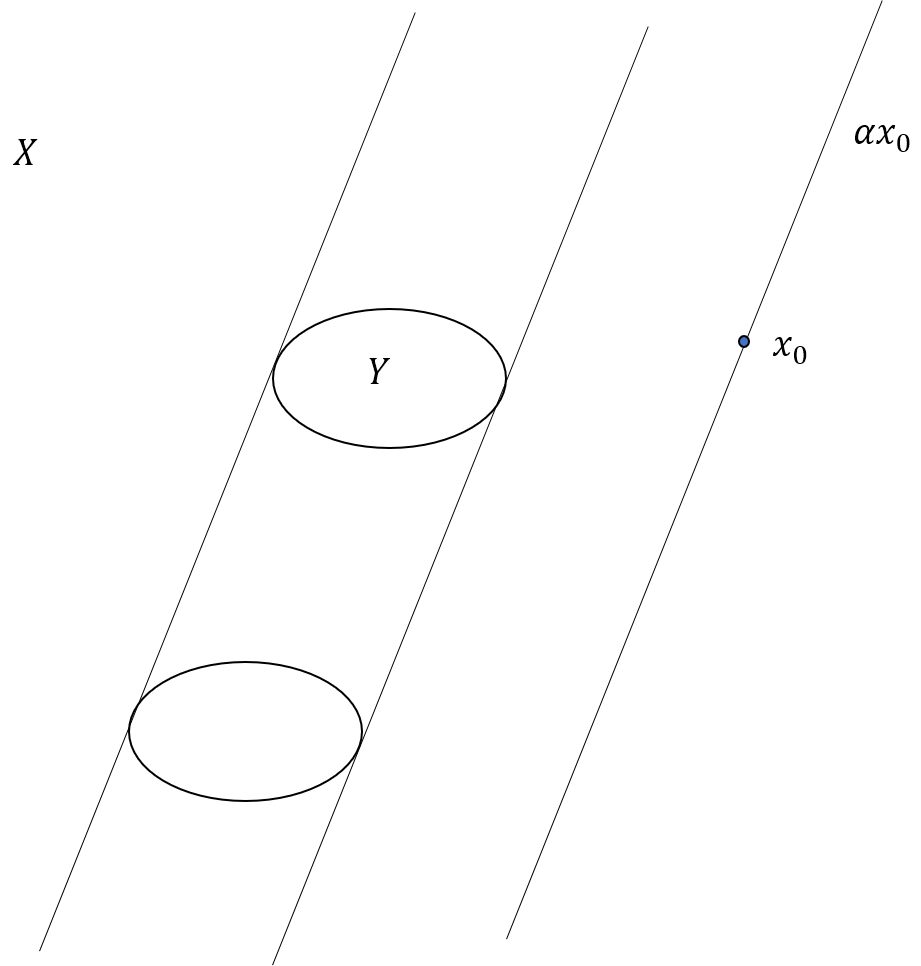
\includegraphics[width=0.5\linewidth]{figure/Domf.png}
\end{center}

(1)局部扩张的存在性.

(构造线性泛函$f\colon\Dom f\rightarrow\mathbb{R}$)现在证明存在线性泛函$f:U(x_0)\rightarrow\mathbb{R}$,它满足
\begin{empheq}{align*}
f(y)&=\ell (y),\forall y\in Y\\
f(x)&\leq p(x), \forall x\in\Dom f
\end{empheq}

假设$f$是存在的,那么它满足
\begin{empheq}{align*}
	f(\alpha x_0+y)&=\alpha f(x_0)+f(y)\\
	&=\alpha f(x_0)+\ell(y)\\
	&\leq p(\alpha x_0+y), \forall\alpha\in \mathbb{R},y\in Y
\end{empheq}

当$\alpha=0$时,显然是成立的(所以$f(y)=\ell(y),\forall y\in Y$自动成立).因为$f$是未知的,假如我们找到一个常数$\lambda\coloneqq f(x_0)$,即令
$$	f(\alpha x_0+y)=\alpha \lambda +\ell(y)$$

这就是一个线性泛函.需要它满足约束,因此现在来确定$\lambda$.
\begin{empheq}{align*}
&\alpha \lambda +\ell(y)\leq p(\alpha x_0+y)\\
\implies & \begin{aligned}[t]
	\lambda &\leq \frac{1}{\alpha}(p(\alpha x_0+y)-\ell y) ,\forall \alpha>0\\
	&=p\left(x_0+\frac{1}{\alpha}y\right)-\ell\left(\frac{1}{\alpha}y\right)
\end{aligned}
\end{empheq}

同时
\begin{empheq}{align*}
	&\alpha \lambda +\ell(y)\leq p(\alpha x_0+y)\\
	\implies & \begin{aligned}[t]
		\lambda &\geq \frac{1}{\alpha}(p(\alpha x_0+y)-\ell y) ,\forall \alpha<0\\
		&=\frac{1}{\alpha}\left(p\left(-\alpha\left(-x_0-\frac{1}{\alpha}y\right)\right)-\ell(y)\right)\\
		&=-p\left(-x_0-\frac{1}{\alpha}y\right)+\ell\left(-\frac{1}{\alpha}y\right)
	\end{aligned}
\end{empheq}

我们已经确定了$\lambda$潜在的上下界,现在还需要确定上界大于下界.由$\ell$的线性和$p$的次线性有
\begin{empheq}{align*}
\ell(u)+\ell(v) &=\ell(u+v),\forall u,v\in Y\\
\leq p(u+v)&=p(-x_0+u+x_0+v)\\
&\leq p(-x_0+u)+p(x_0+v)\\
\implies -p(x_0+u)+\ell(u)&\leq p(x_0+v)-\ell(v)
\end{empheq}

所以可以确定上界确实大于下界.那么取
\begin{empheq}{align*}
a\leq&\lambda\leq b\\
a&\coloneqq \sup_{u\in Y}\{-p(x_0+u)+\ell(u)\}\\
\leq b& \coloneqq \sup_{v\in Y}\{p(x_0+v)-\ell(v)\}
\end{empheq}

即可.

注意把$u,v$对应上去,实际上$u=-\frac{1}{\alpha}y$.

现在回头看思路,实际上构造的泛函是$h(x_0)=f(\alpha x_0+y)=\alpha \lambda +\ell(y)$,即对每个$x_0$有一个函数.反算回去,$\forall x\in U(x_0)$,它满足$f(x)\leq p(x)$.

(2)全局延拓的存在性.

(构造泛函集合)记$\mathcal{F}$为所有满足以下条件的泛函$f:\Dom f\rightarrow \mathbb{R}$的集合:
\begin{empheq}{align*}
f(y)&=\ell(y),\forall y\in Y\\
f(x)&\leq p(x),\forall y\in \Dom f
\end{empheq}

注意$y\subset \Dom f$,且$\Dom f$并非一个固定的子空间.

集合$\mathcal{F}$是非空的,因为$\ell\in \mathcal{F}$.此外,$\mathcal{F}$按以下关系$\preccurlyeq$是半序的:
$$f_1 \preccurlyeq f_2\iff \Dom f_1\subset \Dom f_2, f_2(x)=f_1(x),\forall x\in \Dom f_1$$

关系$\preccurlyeq$实际上就是延拓.

(证明全序子集有上界)给定一个$\mathcal{F}$的一个全序子集$\mathcal{E}$,令
$$\Dom g\coloneqq \bigcup_{f\in \mathcal{E}}\Dom f$$

它显然是$X$的子空间.以下证明,对于$\forall x\in \Dom g$,关系式
$$g(x)\coloneqq f(x), \forall x\in \Dom f, f\in \mathcal{E}$$

\circled{1}定义了一个线性泛函$g\colon \Dom g\rightarrow \mathbb{R}$,\circled{2}且$\forall x\in\Dom g,g(x)\leq p(x)$.

设$x\in \Dom g$使得$x\in \Dom f_1,x\in \Dom f_2$,而$f_1,f_2\in\mathcal{E}$,不妨设$f_1\preccurlyeq f_2$,因此
$$g(x)=f_1(x)=f_2(x)\leq p(x)$$

这证明了第二点.

又假如$x_1\in\Dom f_1,x_2\in\Dom f_2,f_1\preccurlyeq f_2$,那么$x_1+x_2\in\Dom f_2$(实际上$x_1$同时也属于$f_2$).因此$g(x_1+x_2)=f_2(x_1+x_2)=f_2(x_1)+f_2(x_2)=g(x_1)+g(x_2)$.同样地,$\forall \alpha \in \mathbb{R},g(\alpha x_1)=f_1(\alpha x_1)=\alpha f_1(x_1)=\alpha g(x_1)$.

这证明了第二点.

以上说明$g$是$\mathcal{E}$的上界.这是因为$\forall f\in \mathcal{E},\Dom f\subset \Dom g$.

(选择极大元)由Zorn引理,集合$\mathcal{F}$有极大元$\widetilde{\ell}$,它定义在子空间$\Dom \widetilde{\ell}$上.然后有
$$\Dom \widetilde{\ell}=X$$

这就是说$\widetilde{\ell}$正是我们想要找到的泛函.如果$\Dom \widetilde{\ell}\subsetneqq X$,那么可以像第(1)部分一样继续扩张,构造泛函$\widetilde{f}\colon \Dom \widetilde{f}\rightarrow \mathbb{R}$,它满足
$$\Dom \widetilde{\ell}\subsetneqq \Dom \widetilde{f},\widetilde{f}(y)=\ell(y),\forall y\in Y$$
$$\widetilde{f}\leq p(x),\forall x\in \Dom \widetilde{f}$$

这说明$\widetilde{\ell}$不是极大元,矛盾.

因此原命题得证.

\end{proof}

在这个证明中,我们首先进行局部延拓,再通过选择极大元延拓到全局.

